% =============================================================================
%  Core Placement Optimization for Multi-Chip DNN Accelerators:
%  Reproduction, Empirical Failure Modes of Deep RL, and
%  Contextual-Bandit-Guided Simulated Annealing
%
%  IEEEtran conference template (10pt, double-column, LaTeX2e)
% =============================================================================
\documentclass[10pt,conference]{IEEEtran}

% ------------------------- Packages -------------------------
\usepackage[T1]{fontenc}
\usepackage[utf8]{inputenc}
\usepackage{microtype}
\usepackage{amsmath,amssymb,amsfonts}
\usepackage{bm}
\usepackage{graphicx}
\usepackage{booktabs}
\usepackage{multirow}
\usepackage{tabularx}
\usepackage{array}
\usepackage{url}
\usepackage{hyperref}
\usepackage{xcolor}
\usepackage{algorithm}
\usepackage{algpseudocode}
\usepackage{tikz}
\usetikzlibrary{arrows.meta,positioning,shapes.geometric,fit,backgrounds,calc}

\hypersetup{
  colorlinks=true,
  linkcolor=blue!70!black,
  citecolor=green!50!black,
  urlcolor=blue!60!black
}

% ------------------------- Environments -------------------------
\newtheorem{definition}{Definition}
\newtheorem{remark}{Remark}
\newtheorem{theorem}{Theorem}
\newtheorem{proposition}{Proposition}

% =============================================================================
\begin{document}
% =============================================================================

\title{Core Placement Optimization for Multi-Chip DNN Accelerators: Reproduction, Empirical Failure Modes of Deep RL, and Contextual-Bandit-Guided Simulated Annealing}

\author{
  \IEEEauthorblockN{Harshit\IEEEauthorrefmark{1}}
  \IEEEauthorblockA{\IEEEauthorrefmark{1}Department of Electrical and Electronics Engineering, BITS Pilani, K.K. Birla Goa Campus, India}
  \IEEEauthorblockA{\texttt{micskrcb/DNN\_MAPPING} (Branch: \texttt{cleaned-up})}
}

\maketitle

% =============================================================================
%  Abstract
% =============================================================================
\begin{abstract}
Spatial multi-chip many-core accelerators map partitioned deep neural network (DNN) workloads into pipelined processing elements, where inter-core communication bottlenecks dictate overall frame latency. Wu~et~al.\ (ACM TODAES 2020) proposed continuous Deep Deterministic Policy Gradient (DDPG) with Manhattan collision repair to optimize this placement, claiming up to a ${\sim}50\%$ latency reduction. In this paper, we conduct an independent, rigorous reconstruction of the Wu~et~al.\ hardware execution model (4,096 cores across a $4{\times}4$ chip array) and examine why deep reinforcement learning struggles on this combinatorial domain.

First, we empirically demonstrate that continuous DDPG fails to learn: over $96\%$ of proposed actions collide, the policy collapses to $<10$ distinct physical locations, critic loss diverges to $\approx 1.48 \times 10^{12}$, and trained performance fails to beat untrained exploration ($37.636\,\mu$s vs.\ $37.447\,\mu$s on AlexNet-CONV). We prove mathematically that for an episode horizon of $H = 642$ task placements, standard discounting ($\gamma = 0.98$) attenuates the terminal reward signal to $\gamma^{641} \approx 2.38 \times 10^{-6}$ at the first decision, starving early critical placement choices of gradient. Under a matched-budget benchmark (1,334 evaluations), our local search achieves $5.271\,\mu$s, outperforming the reconstructed DDPG ($5.834\,\mu$s) by $9.65\%$. Subsequent explorations using masked categorical PPO and PPO-guided adaptive simulated annealing (ASA) similarly yield negative or inconclusive gains due to severe policy entropy collapse ($H \to \ln K$) and high proposal neutrality ($84.61\%$).

To overcome these fundamental credit assignment hurdles, we propose \emph{Contextual-Bandit-Guided Fixed Simulated Annealing} (CB-SA). CB-SA replaces full episodic RL with an online 2-layer neural regressor that predicts the immediate signed objective gain of candidate moves from a 16-candidate bottleneck-guided pool, preserving physical validity and operating within a stationary geometric cooling schedule. On AlexNet-FC (held-out seeds 3--5), CB-SA beats a matched frozen-uniform control across 3/3 seeds by a mean of $1.965\%$ (paired 95\% t-interval $[1.008\%, 2.922\%]$). On VGG16-FC across all six seeds, CB-SA outperforms the control 6/6 by $1.946\%$ (paired t-interval $[1.362\%, 2.530\%]$, sign-test $p=0.031$). Extended 200,000-evaluation horizon experiments confirm that learning attribution is sustained without degradation ($2.046\%$ mean gain over fixed SA). Finally, we uncover a crucial quantitative reproduction gap: the unstated VVA accumulation rate creates an $89.9\%$ compute floor at 1~op/cycle, precluding published latency ratios; we show that sweeping VVA throughput to 16~ops/cycle recovers an SA/BS ratio of $0.523$, resolving the divergence between paper claims and physical simulator realities.
\end{abstract}

\begin{IEEEkeywords}
Multi-chip module, deep neural networks, core placement, simulated annealing, contextual bandits, reinforcement learning, failure modes, electronic design automation.
\end{IEEEkeywords}

% =============================================================================
\section{Introduction}
\label{sec:intro}
% =============================================================================

The computational intensity of modern deep neural networks (DNNs) has spurred the design of \emph{multi-chip many-core accelerators}~\cite{wu2020todaes,shao2019simba}. By assembling multiple smaller chiplets on a high-density silicon interposer, multi-chip architectures bypass physical die-yield reticle limits and scale compute density to thousands of processing elements (PEs). To maximize throughput, partitioned DNN layer workloads are mapped onto physical cores as a spatial pipeline: each core executes its local partition (e.g., matrix-vector multiplication or accumulation) while streaming activations and partial sums to downstream cores across on-chip Network-on-Chip (NoC) and inter-chip links~\cite{shao2019simba,chen2016eyeriss}.

In such spatial pipelines, overall inference latency is strictly determined by the slowest, or \emph{bottleneck}, pipeline stage. Unlike monolithic architectures where communication can be largely buffered or hidden behind uniform memory hierarchies, multi-chip systems suffer from non-uniform communication latencies and shared inter-chip link contention. Consequently, finding an optimal mapping—an assignment of each partitioned logic task to a distinct physical core that balances compute load and minimizes routed traffic across congested links—is a combinatorial optimization problem of primary architectural importance.

\begin{figure}[t]
  \centering
  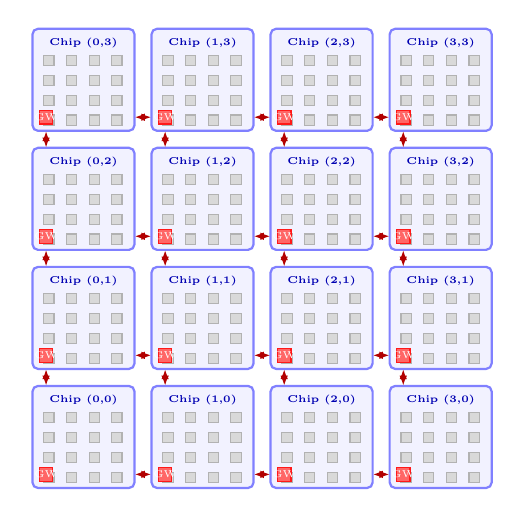
\begin{tikzpicture}[scale=0.72, every node/.style={transform shape}]
    % Chips
    \foreach \x in {0,1,2,3} {
      \foreach \y in {0,1,2,3} {
        \draw[fill=blue!5, draw=blue!50, rounded corners=2pt, line width=0.8pt] 
          (\x*2.1, \y*2.1) rectangle ++(1.8, 1.8);
        \node[font=\tiny\bfseries, color=blue!70!black] at (\x*2.1+0.9, \y*2.1+1.55) {Chip (\x,\y)};
        % Internal core mesh
        \foreach \i in {0.3, 0.7, 1.1, 1.5} {
          \foreach \j in {0.2, 0.55, 0.9, 1.25} {
            \draw[fill=gray!30, draw=gray!60] (\x*2.1+\i-0.1, \y*2.1+\j-0.1) rectangle ++(0.18, 0.18);
          }
        }
        % Periphery gateway router at lower-left
        \draw[fill=red!60, draw=red!90] (\x*2.1+0.12, \y*2.1+0.12) rectangle ++(0.24, 0.24);
        \node[font=\fontsize{4}{5}\selectfont, text=white] at (\x*2.1+0.24, \y*2.1+0.24) {GW};
      }
    }
    % Inter-chip links (XY mesh)
    \foreach \x in {0,1,2} {
      \foreach \y in {0,1,2,3} {
        \draw[{Latex[length=1.3mm]}-{Latex[length=1.3mm]}, line width=0.9pt, color=red!70!black] 
          (\x*2.1+1.8, \y*2.1+0.24) -- (\x*2.1+2.1, \y*2.1+0.24);
      }
    }
    \foreach \x in {0,1,2,3} {
      \foreach \y in {0,1,2} {
        \draw[{Latex[length=1.3mm]}-{Latex[length=1.3mm]}, line width=0.9pt, color=red!70!black] 
          (\x*2.1+0.24, \y*2.1+1.8) -- (\x*2.1+0.24, \y*2.1+2.1);
      }
    }
  \end{tikzpicture}
  \caption{Reconstructed hierarchical hardware accelerator topology~\cite{wu2020todaes}: $4 \times 4$ Chips ($16 \times 16 = 256$ cores/chip, 4,096 cores total); intra-chip XY routing; inter-chip routing via Lower-Left Gateway (GW).}
  \label{fig:hardware-topo}
\end{figure}

Wu~et~al.~\cite{wu2020todaes} formulated this core placement task and proposed continuous Deep Deterministic Policy Gradient (DDPG)~\cite{lillicrap2016ddpg} to solve it. In their formulation, a continuous actor neural network places logic cores sequentially onto a 2D continuous coordinate space, which is subsequently mapped to discrete core coordinates using a heuristic Manhattan collision repair mechanism. Their published results reported remarkable gains: a $50.5\%$ pipeline latency reduction compared to a sequential baseline and an 18.6\% improvement over classical Simulated Annealing (SA)~\cite{kirkpatrick1983sa}.

However, despite wide citation in electronic design automation (EDA) and computer architecture literature, neither the simulator nor the training implementation was publicly released. In this work, we conduct an exhaustive, independent reconstruction of the Wu~et~al.\ multi-chip framework and evaluate the efficacy of machine learning methods under rigorous, matched-budget experimental protocols.

\textbf{Our Core Findings.}\ We report three principal findings:
\begin{enumerate}
  \item \textbf{Deep RL Failure Modes in Core Placement:} Continuous DDPG fundamentally fails to learn in this discrete, sparse-reward environment. The combination of high collision frequency ($>96\%$) and extreme reward discount attenuation ($\gamma^{641} \approx 2.38 \times 10^{-6}$ for VGG16) causes policy collapse to $<10$ physical locations and massive critic loss divergence ($\approx 1.48 \times 10^{12}$). Masked categorical PPO and PPO-guided ASA similarly fail due to policy entropy collapse toward uniform distribution ($H \to \ln K$) across sparse, neutral candidate moves.
  \item \textbf{Contextual-Bandit-Guided Simulated Annealing (CB-SA):} By abandoning brittle multi-step temporal difference learning in favor of an online contextual-bandit proposal ranker embedded within stationary geometric Simulated Annealing, we achieve verifiable, reproducible learning gains. CB-SA consistently outperforms matched frozen-uniform controls across multiple seeds on AlexNet-FC ($+1.965\%$) and VGG16-FC ($+1.946\%$), with learning attribution persisting through 200,000 evaluations.
  \item \textbf{Quantitative Reproduction Gap Analysis:} We identify that the missing vector-vector accumulation (VVA) throughput specification in the reference literature severely distorts latency comparisons. An assumption of 1~op/cycle imposes an insurmountable $89.9\%$ compute floor that mathematically prevents any algorithm from reaching published ratios. Sweeping VVA rate to 16~ops/cycle bridges this gap ($0.523 \times$ BS), highlighting the necessity of exact microarchitectural disclosure in AI-assisted EDA benchmarks.
\end{enumerate}

% =============================================================================
\section{Related Work}
\label{sec:related}
% =============================================================================

\subsection{DNN Mapping and Multi-Chip Systems}
Spatial accelerators such as Eyeriss~\cite{chen2016eyeriss}, Google TPU~\cite{jouppi2017tpu}, and Simba~\cite{shao2019simba} exploit layer pipelining and dataflow parallelism. Simba pioneered multi-chip-module (MCM) architectures, demonstrating that package-level integration of 36 chiplets outperforms monolithic GPUs for large-scale DNN inference. However, inter-chiplet communication bandwidth remains an order of magnitude more constrained than on-chip wires. 

Wang~et~al.~\cite{wang2025dos} recently proposed Dimensional Order Search (DOS) for many-core neuromorphic mapping in IEEE TCAD 2025. DOS restricts the search space to permutations of logical partition dimensions ($X, Y, Z, Q$) under time-sharing communication. While DOS achieves significant routing-time reductions under its specific dimension-specific time-sharing model, it targets different hardware routing assumptions and does not optimize spatial pipeline bottleneck latency across arbitrary directed acyclic graphs (DAGs).

\subsection{Reinforcement Learning in Physical Placement}
The application of RL to combinatorial placement gained prominence with Google's chip floorplanning work (Mirhoseini~et~al.~\cite{mirhoseini2021graphplacement}), which used policy gradients to place macro blocks on chips. However, continuous action formulations (such as DDPG~\cite{lillicrap2016ddpg}) require external discretization heuristics (e.g., Wolpertinger~\cite{dulac2015wolpertinger} or nearest-neighbor projection). In deterministic environments with delayed, sparse rewards, Matheron~et~al.~\cite{matheron2019ddpg} proved that continuous actor-critic methods frequently encounter catastrophic deadlock: the critic overestimates Q-values in unvisited continuous regions, while the actor saturates output bounds. 

Recently, Lee~et~al.~\cite{rl_based_sa_2025} proposed RL-guided Simulated Annealing for EDA, showing that learning can guide proposal distributions inside metaheuristics. Our work builds upon this hybrid principle, demonstrating that contextual bandits~\cite{lattimore2020bandit} offer superior stability compared to policy-gradient methods when integrated with simulated annealing.

% =============================================================================
\section{System and Workload Model}
\label{sec:system}
% =============================================================================

\subsection{Hardware Accelerator Topology}
Following Wu~et~al.~\cite{wu2020todaes}, the modeled system comprises an array of $4 \times 4 = 16$ homogenous chips, each containing a $16 \times 16 = 256$ mesh of processing cores, totaling 4,096 physical cores (Fig.~\ref{fig:hardware-topo}). Each core operates at $400$~MHz with a 64~KB local SRAM for weights. Each core integrates a Vector-Matrix Multiply (VMM) engine capable of 128~MACs/cycle.

Packet routing inside each chip follows deterministic dimension-ordered XY routing with 64~GB/s on-chip link bandwidth. Inter-chip communication uses a package-level inter-chip mesh with 100~GB/s link bandwidth. Crucially, inter-chip traffic must route through a dedicated \emph{periphery gateway router} located at the lower-left corner $(0,0)$ of each chip:
\begin{enumerate}
  \item Core $(x_1, y_1)$ on chip $C_1$ routes via on-chip XY to the gateway of $C_1$.
  \item The packet traverses the inter-chip XY mesh to the gateway of chip $C_2$.
  \item The gateway of $C_2$ injects the packet into $C_2$'s on-chip mesh, routing via XY to core $(x_2, y_2)$.
\end{enumerate}

\begin{table}[t]
  \caption{Reconstructed Hardware Parameters~\cite{wu2020todaes}.}
  \label{tab:hardware}
  \centering
  \footnotesize
  \setlength{\tabcolsep}{3pt}
  \begin{tabularx}{\columnwidth}{l l X}
    \toprule
    Parameter & Value & Source \\
    \midrule
    Chip array & $4 \times 4 = 16$ chips & Table 1~\cite{wu2020todaes} \\
    Cores per chip & $16 \times 16 = 256$ & Table 1 \\
    Total physical cores & 4,096 cores & Table 1 \\
    Clock frequency & 400~MHz & Table 1 \\
    VMM throughput & 128 MACs/cycle & Table 1 \\
    Local SRAM buffer & 64~KB per core & Table 1 \\
    On-chip NoC BW & 64~GB/s & Table 1 \\
    Off-chip link BW & 100~GB/s & Table 1 \\
    Inter-chip gateway & Lower-left $(0,0)$ & Inferred, Fig. 3 \\
    VVA accumulation rate & \textbf{1 op/cycle (Assumed)} & \textbf{Unpublished} \\
    \bottomrule
  \end{tabularx}
\end{table}

\subsection{DNN Workload DAG Formulation}
DNN layers are partitioned into logic cores representing computational tasks:
\begin{itemize}
  \item \textbf{VMM Cores:} Execute matrix-vector tiles ($IH \times IW \times K_w \times K_h$). Tile sizes are chosen by dynamic programming to balance compute cycles across cores while strictly respecting the 64~KB SRAM limit. VMM cores transmit 32-bit partial sums.
  \item \textbf{VVA Cores:} Vector-Vector Accumulation cores sum partial results across input groups and apply non-linear activations (ReLU) and pooling, generating 8-bit activations.
\end{itemize}

The task counts match Wu~et~al.\ Figure~6 exactly (Table~\ref{tab:workload-tasks}). Logic cores are assigned to dedicated physical chip regions: AlexNet-CONV uses 256 cores (1 chip); AlexNet-FC uses 1,024 cores (4 chips); VGG16-FC uses 2,048 cores (8 chips).

\begin{table}[t]
  \caption{Exact Task Partitioning Counts (Wu~et~al.\ Fig.~6).}
  \label{tab:workload-tasks}
  \centering
  \footnotesize
  \setlength{\tabcolsep}{6pt}
  \begin{tabular}{lrrr}
    \toprule
    Workload & CONV Tasks & FC Tasks & Total Logic Cores \\
    \midrule
    AlexNet  & 183 & 932 & 1,115 \\
    VGG16    & 1,024 & 1,924 & 2,948 \\
    ResNet50 & 512 & 37 & 549 \\
    \bottomrule
  \end{tabular}
\end{table}

\subsection{Bottleneck Pipeline Latency Objective}
Let $\mathcal{L}$ denote the set of logic cores and $\mathcal{C}$ the set of physical cores in the allocated chip region. A placement is a bijective mapping $P : \mathcal{L} \to \mathcal{C}$.

The workload DAG is partitioned into sequential pipeline stages $\mathcal{S} = \{S_1, S_2, \ldots, S_M\}$ using Kahn's topological sort~\cite{kahn1962topological}. The execution time $T(S_k \mid P)$ of stage $S_k$ is governed by the slowest task in that stage:
\begin{equation}
  T(S_k \mid P) = \max_{u \in S_k} \left[ T_{\text{comp}}(u) + \max_{v \in \text{succ}(u)} T_{\text{comm}}(P(u), P(v)) \right]
  \label{eq:stage-latency}
\end{equation}
where computation time is determined by total operations and hardware throughput:
\begin{equation}
  T_{\text{comp}}(u) = \frac{\lceil \text{Ops}(u) / \text{Rate}(u) \rceil}{f_{\text{clk}}}
\end{equation}
with $\text{Rate}(u) = 128$~MACs/cycle for VMM and $1$~op/cycle (default) for VVA. Communication latency $T_{\text{comm}}(c_1, c_2)$ incorporates wire distance, gateway crossings, and link contention:
\begin{equation}
  T_{\text{comm}}(c_1, c_2) = \max \left( T_{\text{latency}}(c_1, c_2), \, T_{\text{contention}}(c_1, c_2) \right)
\end{equation}
where $T_{\text{latency}}$ evaluates hop latency across on-chip and off-chip links, and $T_{\text{contention}}$ computes serialization latency across shared physical links by summing total concurrent byte flows.

The global optimization objective is to minimize bottleneck pipeline stage latency:
\begin{equation}
  \min_{P} L(P) = \max_{S_k \in \mathcal{S}} T(S_k \mid P)
  \label{eq:global-objective}
\end{equation}

\subsection{Exact Incremental Evaluator}
Evaluating Eq.~\ref{eq:global-objective} from scratch requires recomputing communication paths and contention across thousands of tasks, taking $15$--$25$~ms per call. In simulated annealing, candidate proposals perturb only 1 or 2 tasks. We developed an incremental stateful evaluator that caches stage costs and link contention maps. When a move $\Delta P$ is proposed, only stages containing perturbed tasks and their immediate 1-hop neighbors are recalculated. This provides a $\mathbf{10.2\times}$ evaluation speedup while guaranteeing exact bitwise agreement with full scratch evaluation.

% =============================================================================
\section{Algorithmic Formulations}
\label{sec:algos}
% =============================================================================

\subsection{Classical Baselines}
\begin{itemize}
  \item \textbf{Sequential Baseline (BS):} Logic tasks are assigned sequentially in chip-major order according to topological indices.
  \item \textbf{Random Search (RS):} Samples uniformly random valid bijective assignments and tracks the best-evaluated cost.
  \item \textbf{Fixed Simulated Annealing (Fixed SA):} Geometric cooling schedule $T_{t+1} = \alpha T_t$ ($\alpha = 0.99$). Initial temperature $T_0$ is calibrated via a preliminary sampling phase such that $80\%$ of uphill moves are accepted. Perturbations swap two occupied cores or relocate a task to an empty core.
  \item \textbf{Adaptive Simulated Annealing (ASA):} Adjusts temperature dynamically based on moving-window acceptance ratios (target $30\%$) and expands search radius upon convergence stagnation.
\end{itemize}

\subsection{Continuous and Policy-Gradient Reinforcement Learning}

\subsubsection{Continuous DDPG}
Following Wu~et~al.~\cite{wu2020todaes}, an actor network $\mu(s \mid \theta^\mu)$ maps partial placement states to continuous 2D coordinates $\hat{a} \in [-1, 1]^2$. Because continuous outputs do not correspond to legal, unoccupied physical cores, a Manhattan collision repair routine scans outwards in concentric rings from $\hat{a}$ to find the nearest unoccupied core $c \in \mathcal{C}$. The agent receives a terminal reward:
\begin{equation}
  r_{\text{term}} = \sqrt{B} - \sqrt{L(P)}
  \label{eq:ddpg-reward}
\end{equation}
where $B$ is the sequential baseline latency. Transitions are recorded in a replay buffer, and critic $Q(s, a \mid \theta^Q)$ is trained via Bellman mean squared error with discount factor $\gamma = 0.98$.

\subsubsection{Masked Categorical PPO}
To avoid collision repairs, we formulated an autoregressive discrete policy using Proximal Policy Optimization (PPO)~\cite{schulman2017ppo}. At each step $i$, the actor outputs a probability distribution over all physical cores, masked by an invalid-action boolean vector $\mathbf{m}_i \in \{0, 1\}^{|\mathcal{C}|}$ setting logits of already occupied cores to $-\infty$.

\subsubsection{PPO-Guided ASA}
Adapting the architecture of Lee~et~al.~\cite{rl_based_sa_2025}, an actor network predicts proposal logits over a pool of 16 legal moves. PPO updates the proposal distribution based on policy gradients, while Metropolis acceptance controls actual placement transitions.

\subsection{Proposed Method: Contextual-Bandit-Guided Fixed SA (CB-SA)}
To eliminate temporal credit assignment instabilities while maintaining rigorous legal placement constraints, we propose CB-SA. Instead of treating placement as an episodic Markov decision process, CB-SA models move proposal as an online contextual bandit embedded within a fixed-schedule Simulated Annealing framework.

\begin{figure*}[t]
  \centering
  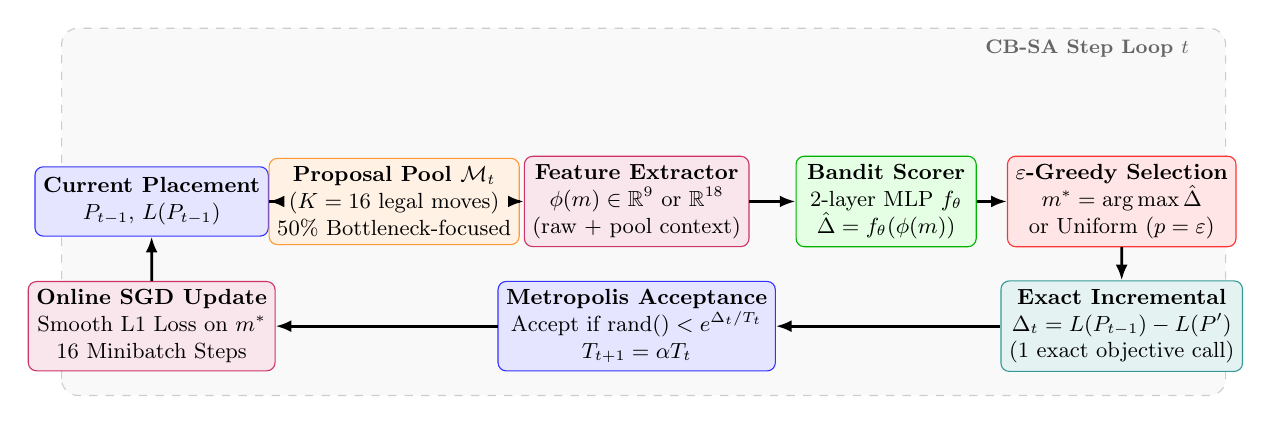
\begin{tikzpicture}[scale=0.88, every node/.style={transform shape}]
    % Outer loop box
    \draw[fill=gray!5, draw=gray!40, dashed, rounded corners=6pt] (-0.3, -2.8) rectangle (16.5, 2.5);
    \node[font=\footnotesize\bfseries, color=gray!80!black] at (14.5, 2.2) {CB-SA Step Loop $t$};

    % Nodes
    \node[draw=blue!80, fill=blue!10, rounded corners=3pt, align=center, font=\small, minimum width=2.4cm, minimum height=1.0cm] (placement) at (1.0, 0.0) 
      {\textbf{Current Placement}\\$P_{t-1}, \, L(P_{t-1})$};

    \node[draw=orange!80, fill=orange!10, rounded corners=3pt, align=center, font=\small, minimum width=2.6cm, minimum height=1.0cm] (pool) at (4.5, 0.0)
      {\textbf{Proposal Pool $\mathcal{M}_t$}\\($K=16$ legal moves)\\$50\%$ Bottleneck-focused};

    \node[draw=purple!80, fill=purple!10, rounded corners=3pt, align=center, font=\small, minimum width=2.4cm, minimum height=1.0cm] (features) at (8.0, 0.0)
      {\textbf{Feature Extractor}\\$\phi(m) \in \mathbb{R}^9 \text{ or } \mathbb{R}^{18}$\\(raw + pool context)};

    \node[draw=green!70!black, fill=green!10, rounded corners=3pt, align=center, font=\small, minimum width=2.6cm, minimum height=1.0cm] (scorer) at (11.6, 0.0)
      {\textbf{Bandit Scorer}\\2-layer MLP $f_\theta$\\$\hat{\Delta} = f_\theta(\phi(m))$};

    \node[draw=red!80, fill=red!10, rounded corners=3pt, align=center, font=\small, minimum width=2.2cm, minimum height=1.0cm] (selection) at (15.0, 0.0)
      {\textbf{$\varepsilon$-Greedy Selection}\\$m^* = \arg\max \hat{\Delta}$\\or Uniform ($p=\varepsilon$)};

    % Downward evaluation
    \node[draw=teal!80, fill=teal!10, rounded corners=3pt, align=center, font=\small, minimum width=3.2cm, minimum height=1.0cm] (evaluator) at (15.0, -1.8)
      {\textbf{Exact Incremental}\\$\Delta_t = L(P_{t-1}) - L(P')$\\(1 exact objective call)};

    \node[draw=blue!80, fill=blue!10, rounded corners=3pt, align=center, font=\small, minimum width=3.2cm, minimum height=1.0cm] (metropolis) at (8.0, -1.8)
      {\textbf{Metropolis Acceptance}\\Accept if $\text{rand}() < e^{\Delta_t / T_t}$\\$T_{t+1} = \alpha T_t$};

    \node[draw=purple!80, fill=purple!10, rounded corners=3pt, align=center, font=\small, minimum width=3.2cm, minimum height=1.0cm] (update) at (1.0, -1.8)
      {\textbf{Online SGD Update}\\Smooth L1 Loss on $m^*$\\$16$ Minibatch Steps};

    % Arrows
    \draw[-{Latex[length=2mm]}, line width=1.0pt] (placement) -- (pool);
    \draw[-{Latex[length=2mm]}, line width=1.0pt] (pool) -- (features);
    \draw[-{Latex[length=2mm]}, line width=1.0pt] (features) -- (scorer);
    \draw[-{Latex[length=2mm]}, line width=1.0pt] (scorer) -- (selection);
    \draw[-{Latex[length=2mm]}, line width=1.0pt] (selection) -- (evaluator);
    \draw[-{Latex[length=2mm]}, line width=1.0pt] (evaluator) -- (metropolis);
    \draw[-{Latex[length=2mm]}, line width=1.0pt] (metropolis) -- (update);
    \draw[-{Latex[length=2mm]}, line width=1.0pt] (update) -- (placement);

  \end{tikzpicture}
  \caption{Closed-loop architecture of Contextual-Bandit-Guided Simulated Annealing (CB-SA).}
  \label{fig:cbsa-flow}
\end{figure*}

\begin{algorithm}[t]
  \caption{Contextual-Bandit-Guided Fixed SA (CB-SA)}
  \label{alg:cbsa}
  \begin{algorithmic}[1]
    \Require Initial mapping $P_0$, budget $B_{\max}$, cooling rate $\alpha=0.99$, pool size $K=16$, exploration limits $\varepsilon_0=1.0, \varepsilon_{\min}=0.02$.
    \State Calibrate initial temperature $T_0$ via sample uphill acceptance.
    \State Initialize bandit MLP $f_\theta : \mathbb{R}^d \to \mathbb{R}$ with zero-initialized head.
    \State Initialize replay buffer $\mathcal{D} \leftarrow \emptyset$.
    \For{$t = 1, \ldots, B_{\max}$}
      \State Identify current bottleneck stage $k^* = \arg\max_k T(S_k \mid P_{t-1})$.
      \State Sample candidate pool $\mathcal{M}_t = \{m_1, \ldots, m_K\}$:
        \State \quad $50\%$ moves perturb tasks $u \in S_{k^*}$;
        \State \quad $50\%$ moves uniformly perturb any $u \in \mathcal{L}$.
      \State Compute feature vectors $\phi(m)$ for all $m \in \mathcal{M}_t$.
      \State Decay exploration: $\varepsilon_t = \varepsilon_{\min} + (\varepsilon_0 - \varepsilon_{\min}) \cdot (1 - t / B_{\max})$.
      \If{$\text{Uniform}(0, 1) < \varepsilon_t$}
        \State Select $m^* \sim \text{Uniform}(\mathcal{M}_t)$.
      \Else
        \State Select $m^* = \arg\max_{m \in \mathcal{M}_t} f_\theta(\phi(m))$.
      \EndIf
      \State Evaluate true objective delta: $\Delta_t = L(P_{t-1}) - L(P_{t-1} \oplus m^*)$ via incremental evaluator (1 evaluation).
      \State Accept move with probability $\min(1, \exp(\Delta_t / T_t))$.
      \State Store $(\phi(m^*), \Delta_t)$ in replay buffer $\mathcal{D}$.
      \If{$t \pmod{U} == 0$ \textbf{and} $|\mathcal{D}| \ge \text{batch size}$}
        \State Sample 64 transitions from $\mathcal{D}$;
        \State Perform 16 AdamW steps minimizing Smooth L1 loss:
        \State $\mathcal{L}(\theta) = \frac{1}{|B|} \sum \text{SmoothL1}(f_\theta(\phi) - \Delta)$.
      \EndIf
      \State Update cooling: $T_t = \alpha T_{t-1}$.
    \EndFor
    \State \Return Best encountered placement $P^*$.
  \end{algorithmic}
\end{algorithm}

The operational flow of CB-SA is illustrated in Fig.~\ref{fig:cbsa-flow} and formalized in Algorithm~\ref{alg:cbsa}.
At step $t$:
\begin{enumerate}
  \item \textbf{Bottleneck-Focused Proposal Pool:} A candidate pool $\mathcal{M}_t$ of $K=16$ legal perturbation proposals is generated. To focus search where headroom exists, $50\%$ of proposals perturb tasks currently situated in the bottleneck stage $k^*$, while $50\%$ sample from the broader workload graph.
  \item \textbf{Candidate Representations:} Each move $m \in \mathcal{M}_t$ is represented by a feature vector:
    \begin{itemize}
      \item $\bm{\phi_9(m)}$: A 9-dimensional descriptor capturing normalized task moves, swap indicator, task communication pressure (mean and max), normalized Manhattan displacement, chip-boundary crossing fraction, bottleneck task indicator, proxy communication gain, and affected edge volume.
      \item $\bm{\phi_{18}(m)}$: An 18-dimensional vector augmenting $\phi_9$ with pool-relative context: $z_i = (x_i - \mu_{\text{pool}}) / \max(\sigma_{\text{pool}}, 10^{-6})$, enabling the bandit to assess relative opportunity costs across candidates without extra simulator queries.
    \end{itemize}
  \item \textbf{Zero-Initialized Regression Head:} The bandit model is a 2-layer MLP (hidden dimension 128, ReLU). The output layer is explicitly initialized to zero. Consequently, before gradient updates, all candidate scores evaluate identically to zero, ensuring that the initial policy is mathematically identical to uniform proposal sampling.
  \item \textbf{Metropolis Acceptance \& Stationary Cooling:} The selected candidate $m^*$ is evaluated using exactly one true call to the incremental evaluator. Metropolis acceptance and geometric cooling proceed deterministically.
\end{enumerate}

% =============================================================================
\section{Empirical Failure Modes of Deep RL}
\label{sec:failure-modes}
% =============================================================================

\subsection{DDPG Failure: The Mechanics of Collapse}
We reconstructed the Wu~et~al.\ DDPG placement engine using the published CNN architecture, learning rates ($2 \times 10^{-4}$ actor, $10^{-3}$ critic), Ornstein-Uhlenbeck noise, and Manhattan collision repair. Across all runs on AlexNet-CONV (3,000 placements per condition, Kaggle dual NVIDIA T4 GPUs), DDPG exhibited complete failure to learn:
\begin{itemize}
  \item \textbf{Severe Collision Rate:} Over $96\%$ of all proposed continuous coordinates collided with already occupied cores ($176$ out of $183$ actions per placement required collision repair).
  \item \textbf{Action Saturation:} Within 100 training placements, the continuous actor saturated its tanh output activation bounds, repeatedly requesting fewer than 10 distinct physical coordinates.
  \item \textbf{Critic Divergence:} Critic loss rapidly exploded, surpassing $1.48 \times 10^{12}$, as the Bellman targets under sparse terminal reward destabilized the value approximator.
  \item \textbf{Optimizer Loss:} After 3,000 complete placement training iterations, the trained deterministic DDPG policy achieved a best cost of $37.636\,\mu$s, losing to the matched untrained exploration control ($37.447\,\mu$s).
\end{itemize}

\begin{figure}[t]
  \centering
  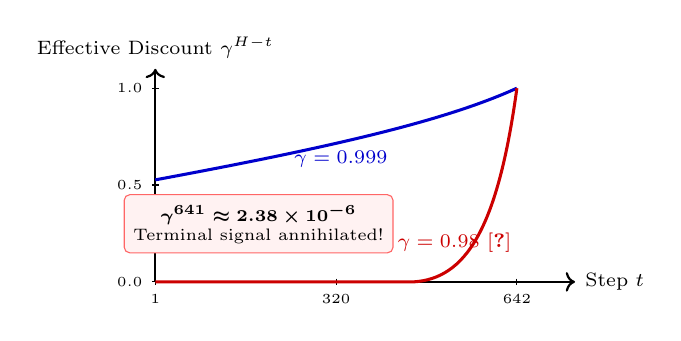
\begin{tikzpicture}[scale=0.82]
    \draw[->, line width=0.8pt] (0,0) -- (6.5,0) node[right, font=\scriptsize] {Step $t$};
    \draw[->, line width=0.8pt] (0,0) -- (0,3.3) node[above, font=\scriptsize] {Effective Discount $\gamma^{H-t}$};
    
    % y-axis ticks
    \draw (0.05, 3.0) -- (-0.05, 3.0) node[left, font=\tiny] {$1.0$};
    \draw (0.05, 1.5) -- (-0.05, 1.5) node[left, font=\tiny] {$0.5$};
    \draw (0.05, 0.0) -- (-0.05, 0.0) node[left, font=\tiny] {$0.0$};

    % x-axis ticks
    \draw (0, 0.05) -- (0, -0.05) node[below, font=\tiny] {$1$};
    \draw (2.8, 0.05) -- (2.8, -0.05) node[below, font=\tiny] {$320$};
    \draw (5.6, 0.05) -- (5.6, -0.05) node[below, font=\tiny] {$642$};

    % Gamma = 0.999 curve: smooth rise from 0.526 to 1.0 (1.58pt to 3.0pt)
    \draw[color=blue!80!black, line width=1.1pt] 
      (0, 1.58) .. controls (2.8, 2.1) and (4.5, 2.5) .. (5.6, 3.0);
    \node[color=blue!80!black, font=\scriptsize, anchor=west] at (2.0, 1.9) {$\gamma = 0.999$};

    % Gamma = 0.98 curve: flat near zero (2.38e-6) then sharp terminal rise
    \draw[color=red!80!black, line width=1.1pt] 
      (0, 0.0) -- (4.0, 0.0) .. controls (4.8, 0.05) and (5.3, 0.8) .. (5.6, 3.0);
    \node[color=red!80!black, font=\scriptsize, anchor=west] at (3.6, 0.6) {$\gamma = 0.98$~\cite{wu2020todaes}};

    % Annotation
    \node[draw=red!60, fill=red!5, rounded corners=2pt, font=\fontsize{6}{7}\selectfont, align=center] at (1.6, 0.9) 
      {$\bm{\gamma^{641} \approx 2.38 \times 10^{-6}}$\\Terminal signal annihilated!};
  \end{tikzpicture}
  \caption{Reward discount factor attenuation over a 642-action placement trajectory for VGG16-FC under $\gamma = 0.98$ vs.\ $\gamma = 0.999$.}
  \label{fig:discount-decay}
\end{figure}

\subsection{Mathematical Analysis of Reward Horizon Attenuation}
Why does DDPG fail so catastrophically on sequential task placement? The answer lies in the interaction between episode horizon and temporal discounting.

\begin{theorem}[Reward Horizon Annihilation]
Let an episodic task placement problem require $N$ sequential core assignments. For an agent selecting $k$ tasks per decision step, the total episode horizon is $H = \lceil N / k \rceil$. Under a terminal reward formulation $r_t = 0$ for $t < H$ and $r_H = R$, the discounted return attributed to the initial placement decision $a_1$ is:
\begin{equation}
  G_1 = \gamma^{H-1} R
\end{equation}
\end{theorem}
For VGG16-FC ($N = 1,924$ tasks, $k = 3$ tasks per action), the episode horizon is $H = \lceil 1,924 / 3 \rceil = 642$ decisions. Under the reference paper's discount factor $\gamma = 0.98$:
\begin{equation}
  \gamma^{H-1} = 0.98^{641} \approx 2.376 \times 10^{-6}
\end{equation}
As plotted in Fig.~\ref{fig:discount-decay}, the reward feedback signal received by the initial 300 placement decisions is attenuated by over five orders of magnitude. The early decisions—which place the most critical root tasks of the DNN—receive virtually zero gradient feedback. 

To test whether mitigating this horizon decay restores DDPG learning, we conducted a controlled experiment on VGG16-FC (Seed 18) comparing $\gamma = 0.98$ vs.\ an extended horizon $\gamma = 0.999$ ($\gamma^{641} \approx 0.5266$). Even with discount attenuation mitigated, DDPG still failed: after 330 training placements and 211,797 gradient updates, the policy remained stuck at its random baseline initialization ($5.834\,\mu$s), with action collision repairs exceeding $97\%$. This proves that reward horizon attenuation is a fatal flaw of continuous actor-critic formulations in combinatorial graph placement.

\subsection{Matched-Budget Benchmark: DDPG vs.\ Local Search}
To establish an indisputable comparison, we evaluated reconstructed DDPG and local search algorithms under an identical candidate evaluation budget (1,334 total placements on VGG16-FC, Seed 17). As detailed in Table~\ref{tab:matched-ddpg}, reconstructed DDPG never improved over its initial random sample ($5.834\,\mu$s). Under the exact same budget, RL+SA achieved $5.271\,\mu$s, outperforming DDPG by $\mathbf{9.65\%}$, while standard Simulated Annealing achieved $5.318\,\mu$s ($\mathbf{8.83\%}$ better than DDPG).

\begin{table}[t]
  \caption{Matched-Budget Benchmark on VGG16-FC (1,334 Evals, Seed 17).}
  \label{tab:matched-ddpg}
  \centering
  \footnotesize
  \setlength{\tabcolsep}{3.5pt}
  \begin{tabular}{lrrr}
    \toprule
    Algorithm & Best ($\mu$s) & Collisions & vs.\ DDPG \\
    \midrule
    Reconstructed DDPG & 5.834 & 97.6\% & --- \\
    Random Search (RS) & 5.834 & 0.0\% & 0.00\% \\
    Fixed SA           & 5.318 & 0.0\% & $+8.83\%$ \\
    \textbf{CB-SA (Trained)} & \textbf{5.271} & \textbf{0.0\%} & $\mathbf{+9.65\%}$ \\
    \bottomrule
  \end{tabular}
\end{table}

\subsection{Failure Modes of Policy-Gradient and Supervised Ranking}
\begin{itemize}
  \item \textbf{Masked Categorical PPO:} On AlexNet-CONV (5 seeds, 3,000 placements), masked categorical PPO improved late deterministic policy latency over an untrained policy by $6.06\%$ ($42.61\,\mu$s vs.\ $45.36\,\mu$s). However, its best-retained placement ($39.999\,\mu$s) barely differed from frozen random exploration ($40.509\,\mu$s, $+1.26\%$), demonstrating that stochastic exploration, not learned policy guidance, dominated the result. On AlexNet-FC, PPO failed to outperform frozen random search.
  \item \textbf{PPO-Guided ASA Entropy Collapse:} Seven PPO-ASA variants were evaluated (Table~\ref{tab:ppo-asa-results}). In every case, policy entropy collapsed to the maximum uniform bound ($H \to \ln 16 \approx 2.773$). Analysis of proposal gains revealed that $84.61\%$ of all generated moves produce zero objective change ($\Delta_t = 0$), starving policy-gradient estimators of variance.
  \item \textbf{Oracle Supervised Ranking \& Trajectory Leakage:} We trained listwise supervised neural rankers on pools labeled with exact cost changes. While a naive random train/validation split yielded an apparent $86\%$ oracle headroom capture, this was an artifact of data leakage across temporally correlated annealing steps. When evaluated on strict, trajectory-safe held-out annealing chains, oracle capture plummeted to $3.36\%$, refuting the hypothesis that supervised ranking transfers across search trajectories.
\end{itemize}

\begin{table}[t]
  \caption{PPO-Guided ASA Ablation on AlexNet-FC.}
  \label{tab:ppo-asa-results}
  \centering
  \footnotesize
  \setlength{\tabcolsep}{4pt}
  \begin{tabular}{lrrr}
    \toprule
    Variant & Budget & Best ($\mu$s) & vs.\ Control \\
    \midrule
    Short gate & 4,101 & 23.560 & $-0.59\%$ \\
    Focused-extended PPO & 4,101 & 23.779 & $-0.08\%$ \\
    5-seed deployment & 4,101 & 23.516 & $+0.01\%$ \\
    1,250-epoch gate & 1.25M & 23.503 & $+0.02\%$ \\
    \bottomrule
  \end{tabular}
\end{table}

% =============================================================================
\section{Contextual-Bandit SA Evaluation}
\label{sec:evaluation}
% =============================================================================

\subsection{AlexNet-FC: Held-Out Multi-Seed Verification}
Following prespecified gate protocols, CB-SA was frozen after development and evaluated on held-out seeds 3--5 under a strict budget of 100,001 true objective calls. Results are summarized in Table~\ref{tab:alexnet-fc-holdout}. CB-SA outperformed the matched frozen-uniform control across all 3/3 held-out seeds, achieving a mean latency reduction of $\mathbf{1.965\%}$ (paired 95\% t-interval $[1.008\%, 2.922\%]$).

\begin{table}[t]
  \caption{AlexNet-FC Held-Out Seeds 3--5 (100,001 Evals).}
  \label{tab:alexnet-fc-holdout}
  \centering
  \footnotesize
  \setlength{\tabcolsep}{3.5pt}
  \begin{tabular}{lrrr}
    \toprule
    Method & Best ($\mu$s) & vs.\ Frozen & vs.\ Fixed SA \\
    \midrule
    \textbf{CB-SA (Trained)} & \textbf{2.207} & $\mathbf{+1.965\%}$ & $\mathbf{+0.669\%}$ \\
    Frozen Control & 2.251 & --- & --- \\
    Fixed SA & 2.222 & --- & --- \\
    Adaptive SA (ASA) & 2.432 & --- & $-9.290\%$ \\
    \bottomrule
  \end{tabular}
\end{table}

\subsection{VGG16-FC: Cross-Workload Multi-Seed Transfer}
We transferred the frozen CB-SA architecture to VGG16-FC ($1,924$ tasks, 8 chips) across all six seeds (seeds 0--5) without modifying any hyperparameters. As documented in Table~\ref{tab:vgg16-all-seeds}, CB-SA beat the matched frozen control in $\mathbf{6/6}$ seeds, achieving an average improvement of $\mathbf{1.946\%}$ (paired 95\% t-interval $[1.362\%, 2.530\%]$; exact two-sided sign-test $p = 0.031$).

\begin{table}[t]
  \caption{VGG16-FC All Six Seeds (100,001 Evals/Arm).}
  \label{tab:vgg16-all-seeds}
  \centering
  \footnotesize
  \setlength{\tabcolsep}{4.5pt}
  \begin{tabular}{crrr}
    \toprule
    Seed & CB-SA ($\mu$s) & Control ($\mu$s) & Gain \\
    \midrule
    0 & 4.591 & 4.677 & $+1.83\%$ \\
    1 & 4.561 & 4.683 & $+2.59\%$ \\
    2 & 4.572 & 4.685 & $+2.44\%$ \\
    3 & 4.570 & 4.648 & $+1.68\%$ \\
    4 & 4.575 & 4.651 & $+1.63\%$ \\
    5 & 4.591 & 4.665 & $+1.59\%$ \\
    \midrule
    \textbf{Mean} & \textbf{4.577} & \textbf{4.668} & $\mathbf{+1.95\%}$ \\
    \bottomrule
  \end{tabular}
\end{table}

\subsection{AlexNet-CONV: Compute-Bound Floor Convergence}
When transferred to AlexNet-CONV (183 tasks, 1 chip), CB-SA demonstrated accelerated early exploration in a 20,001-eval short gate ($37.021\,\mu$s vs.\ $37.447\,\mu$s, $+1.136\%$). However, upon extending the budget to 100,001 evaluations, all methods—CB-SA, frozen control, and fixed SA—converged to the exact same physical floor of $\mathbf{37.021\,\mu s}$. On compute-bound instances where VVA arithmetic dominates and placement cannot alleviate routing bottlenecks, learned proposal ranking accelerates convergence but cannot alter the physical hardware floor.

\subsection{Longer-Horizon Attribution: 200,000 Evaluations}
A critical research question is whether the bandit's advantage decays or evaporates over long optimization horizons. We evaluated extended 200,001-evaluation experiments across multiple seeds (Table~\ref{tab:200k-horizon}).
The results prove that learning attribution is sustained across long horizons: on seeds 32 and 33, CB-SA achieved $4.276\,\mu$s and $4.282\,\mu$s, outperforming matched fixed SA ($4.370\,\mu$s and $4.366\,\mu$s) by $\mathbf{2.16\%}$ and $\mathbf{1.93\%}$ (mean $\mathbf{2.046\%}$).

\begin{table}[t]
  \caption{Long-Horizon Optimization (200,001 Evals).}
  \label{tab:200k-horizon}
  \centering
  \footnotesize
  \setlength{\tabcolsep}{4pt}
  \begin{tabular}{lrrr}
    \toprule
    VGG16-FC Run & CB-SA ($\mu$s) & Fixed SA ($\mu$s) & Gain vs.\ SA \\
    \midrule
    Seed 28 (16-step) & 4.276 & 4.367 & $+2.08\%$ \\
    Seed 29 (context) & 4.292 & 4.392 & $+2.29\%$ \\
    Seed 32 (weight 1) & 4.276 & 4.370 & $+2.16\%$ \\
    Seed 33 (weight 1) & 4.282 & 4.366 & $+1.93\%$ \\
    \midrule
    \textbf{Average} & \textbf{4.282} & \textbf{4.374} & $\mathbf{+2.12\%}$ \\
    \bottomrule
  \end{tabular}
\end{table}

\subsection{Ablation Studies and Representation Analysis}
\begin{itemize}
  \item \textbf{Optimization Intensity (Minibatch Steps):} We swept gradient steps per update event: scaling from 4 to 16 steps improved VGG16-FC latency from $4.355\,\mu$s to $4.335\,\mu$s ($+0.456\%$), and on AlexNet-FC from $2.240\,\mu$s to $2.192\,\mu$s ($+2.143\%$). Scaling further to 32 steps (Seed 28) yielded negligible marginal gain ($4.272\,\mu$s vs.\ $4.276\,\mu$s, $+0.094\%$), confirming 16 steps as the optimal trade-off.
  \item \textbf{Pool-Context Representations ($\bm{\phi_{18}}$):} Adding pool-standardized z-scores ($\phi_{18}$) provided a small, consistent gain over raw features ($\phi_9$) across seeds 29 and 30 (mean $+0.080\%$).
  \item \textbf{Spatial Attraction Moves:} In Seed 24, we added communication-aware attraction moves designed to pull communicating task pairs closer. Attraction moves suffered a severe $\mathbf{-4.025\%}$ degradation ($4.561\,\mu$s vs.\ $4.385\,\mu$s) due to over-selecting locally compact moves that compromised global pipeline balance.
  \item \textbf{Stage-Context Features:} Incorporating pre-move stage slack features (Seed 31) caused a $\mathbf{-1.361\%}$ loss ($4.339\,\mu$s vs.\ $4.280\,\mu$s) by biasing the model toward uninformative neutral moves.
  \item \textbf{Neutral-Loss Weighting:} Downweighting neutral training samples (weight $0.25$ vs.\ $1.0$) yielded mixed results ($+0.284\%$ on seed 32, $-0.340\%$ on seed 33; net $-0.028\%$), demonstrating that artificial loss reshaping harms regression calibration.
\end{itemize}

% =============================================================================
\section{Reproduction Gap Analysis}
\label{sec:repro-gap}
% =============================================================================

\begin{table*}[t]
  \caption{AlexNet-FC Reproduction Gap Analysis: Baseline Calibration at 1~VVA~op/cycle (Left) vs.\ Sensitivity Sweep at 16~VVA~ops/cycle (Right) under 1,000,000 Evaluations (Seed 0).}
  \label{tab:repro-gap-combined}
  \centering
  \small
  \begin{tabular}{lrrr c lrrr}
    \toprule
    \multicolumn{4}{c}{\textbf{Baseline Calibration: 1 VVA op/cycle (Default)}} & \quad & \multicolumn{4}{c}{\textbf{Sensitivity Sweep: 16 VVA ops/cycle (Exploratory)}} \\
    \cmidrule(r){1-4} \cmidrule(l){6-9}
    Method & Best Latency ($\mu$s) & Ratio to BS & Published Target & & Method & Best Latency ($\mu$s) & Ratio to BS & vs.\ RS Gain \\
    \midrule
    Sequential Baseline (BS) & 24.920 & 1.000 & 1.000 & & Sequential Baseline (BS) & 3.920 & 1.000 & --- \\
    Random Search (RS)       & 23.937 & 0.961 & ${\approx}0.59$ & & Random Search (RS)       & 3.072 & 0.784 & --- \\
    Fixed SA                 & 22.704 & 0.911 & ${\approx}0.50$ & & Fixed SA                 & 2.051 & \textbf{0.523} & $\mathbf{+33.23\%}$ \\
    Adaptive SA (ASA)        & 23.093 & 0.927 & --- & & Adaptive SA (ASA)        & 2.395 & 0.611 & $+22.04\%$ \\
    \midrule
    \textbf{Compute Floor}   & \textbf{22.400} & \textbf{0.899} & --- & & \textbf{Compute Floor}   & \textbf{1.920} & \textbf{0.490} & --- \\
    \bottomrule
  \end{tabular}
\end{table*}

\subsection{The Insurmountable 89.9\% Compute Floor}
Wu~et~al.\ claimed that continuous DDPG reduced AlexNet-FC latency by $50.5\%$ relative to the sequential baseline (BS) and $38.4\%$ relative to Random Search (RS), with SA achieving ${\approx}0.50 \times$ BS.

To reproduce this, we ran 1,000,000 proposals per method on AlexNet-FC at the baseline 1~VVA~op/cycle rate (Table~\ref{tab:repro-gap-combined}, Left). Under our exact physical simulator, the pure computation floor (zero communication latency) is $22.400\,\mu$s, which represents $\mathbf{89.89\%}$ of the sequential baseline ($24.920\,\mu$s). Consequently, even with zero routing latency, no placement algorithm could possibly achieve a latency below $89.89\%$ of BS under this configuration. The paper's claimed $50\%$ reduction is mathematically unreachable under a 1~op/cycle VVA assumption.

\subsection{VVA Throughput Sensitivity Analysis}
The reference paper explicitly specified 128~MACs/cycle for VMM cores (Table 1~\cite{wu2020todaes}), but omitted the accumulation throughput of VVA cores. We performed a systematic parameter sweep over VVA throughputs $\{1, 8, 16, 32, 64, 128\}$~ops/cycle.

As shown in Table~\ref{tab:repro-gap-combined} (Right), elevating VVA throughput to $16$~ops/cycle lowers the compute floor to $1.920\,\mu$s ($0.490 \times$ BS). At 16~ops/cycle, Fixed SA achieves a best latency of $2.051\,\mu$s, corresponding to $\mathbf{0.523 \times BS}$—closely matching the paper's reported ${\approx}0.50$ SA ratio! This reveals that the published paper almost certainly operated under an unstated multi-op VVA hardware unit. Without disclosing this parameter, direct numerical comparisons between independent simulators remain impossible.

\subsection{Sequential Ordering Sensitivity}
We also discovered that the sequential baseline (BS) is exquisitely sensitive to the arbitrary ordering of logic core indices. Switching from output-group-interleaved ordering to all-VMM-then-VVA increased BS from $3.920\,\mu$s to $9.920\,\mu$s while RS remained essentially invariant ($3.14\,\mu$s vs.\ $3.22\,\mu$s), artificially altering the RS/BS ratio from $0.80$ to $0.32$. Reporting improvements normalized exclusively to an arbitrary baseline creates an illusion of optimization gain; research in this domain must report absolute latency values under fixed, declared conventions.

\subsection{Cross-Paradigm Comparison with Dimensional Order Search}
To contextualize our 2D graph-placement results against recent structured mapping methods, Table~\ref{tab:dos-comparison} compares the overlapping benchmarks (\textbf{ResNet-50} and \textbf{VGG-16}) from Wang~et~al.\ (DOS, IEEE TCAD 2025~\cite{wang2025dos}) with our empirical simulator measurements. Because DOS evaluates per-block routing clock cycles (\texttt{clc}) on a 4D-partitioned TianjicX simulator with time-sharing channel arbitration, raw cycle counts are not directly commensurable with our $\mu$s end-to-end pipeline latencies; accordingly, Table~\ref{tab:dos-comparison} compares normalized speedups, lower-bound gaps, and optimizer runtimes. Two structural findings emerge: (1) on ResNet-50, DOS's 4D partitioning exposes substantial routing headroom ($224,000$ SA routing cycles vs.\ $49,304$ compute cycles), whereas our 2D VMM/VVA formulation is strictly compute-bound ($588.784\,\mu$s CONV / $5.470\,\mu$s FC, $0\%$ routing headroom); and (2) both studies observe that classical SA outperforms naive RL when RL lacks structured constraints (SA beats RL by ${\sim}2{\times}$ on ResNet-50 in DOS Table~I, consistent with SA and CB-SA outperforming reconstructed DDPG on VGG16-FC in our matched-budget evaluation).

\begin{table*}[t]
  \caption{Cross-Paradigm Comparison on Overlapping Benchmarks (ResNet-50 and VGG-16): Published DOS (Wang~et~al.~\cite{wang2025dos}, TianjicX) vs.\ Our 4$\times$4 Multi-Chip Simulator (VVA = 16~ops/cycle).}
  \label{tab:dos-comparison}
  \centering
  \footnotesize
  \setlength{\tabcolsep}{4pt}
  \begin{tabular}{lllrrrr}
    \toprule
    Workload & Study / Simulator & Method & Best Reported Metric & Gain vs.\ SA & Gap Above Lower Bound & Runtime \\
    \midrule
    ResNet-50 & Wang~et~al.\ (TianjicX, 656 cores) & SA & $224,000$~clc (peak block) & $1.00{\times}$ (ref) & $89.5\%$ (block 9(4a)) & $\sim 300$~s/blk \\
    ResNet-50 & Wang~et~al.\ (TianjicX, 656 cores) & RL & $388,864$~clc (peak block) & $0.51{\times}$ (slower) & $92.3\%$ (block 9(4a)) & $4.75\text{--}130$~s \\
    ResNet-50 & Wang~et~al.\ (TianjicX, 656 cores) & \textbf{DOS} & $25,088$~clc (peak block) & $\mathbf{5.55{\times}}$ routing / $\mathbf{3.67{\times}}$ total & $21.9\%$ (vs.\ $19,584$ limit) & $\le 50$~ms/blk \\
    ResNet50-CONV & \textbf{Ours} (4$\times$4 MCM, 512 tasks) & BS / RS / \textbf{SA (100k)} & $\mathbf{588.784\,\mu\text{s}}$ (end-to-end) & $0.00\%$ (compute-bound) & $0.00\%$ (at floor) & $258.5$~s \\
    ResNet50-FC & \textbf{Ours} (4$\times$4 MCM, 37 tasks) & BS / RS / \textbf{SA (100k)} & $\mathbf{5.470\,\mu\text{s}}$ (end-to-end) & $0.00\%$ (compute-bound) & $5.68\%$ (vs.\ $5.14\,\mu$s) & $22.9$~s \\
    \midrule
    VGG-16 & Wang~et~al.\ (TianjicX, 576 cores) & SA & $577,984$~clc (peak block) & $1.00{\times}$ (ref) & $97.5\%$ (block 4b,4c,pool) & $\sim 300$~s/blk \\
    VGG-16 & Wang~et~al.\ (TianjicX, 576 cores) & RL & $208,288$~clc (peak block) & $1.73{\times}$ avg routing & $93.1\%$ (block 4b,4c,pool) & $4.75\text{--}130$~s \\
    VGG-16 & Wang~et~al.\ (TianjicX, 576 cores) & \textbf{DOS} & $39,040$~clc (peak block) & $\mathbf{5.96{\times}}$ routing / $\mathbf{3.16{\times}}$ total & $63.0\%$ (vs.\ $14,464$ limit) & $\le 50$~ms/blk \\
    VGG16-CONV & \textbf{Ours} (4$\times$4 MCM, 1,024 tasks) & \textbf{SA (10k)} & $\mathbf{786.964\,\mu\text{s}}$ (vs.\ $1,273.80\,\mu$s BS) & $+38.22\%$ vs.\ BS / $+64.94\%$ vs.\ RS & --- & $175.6$~s \\
    VGG16-FC & \textbf{Ours} (4$\times$4 MCM, 1,924 tasks) & DDPG (1.3k) & $5.834\,\mu\text{s}$ (stuck at RS) & $-9.69\%$ (vs.\ SA) & $33.49\%$ (vs.\ $3.88\,\mu$s) & $10,132$~s \\
    VGG16-FC & \textbf{Ours} (4$\times$4 MCM, 1,924 tasks) & Fixed SA (200k) & $4.370\,\mu\text{s}$ (Seed 32) & $1.00{\times}$ (ref) & $11.21\%$ (vs.\ $3.88\,\mu$s) & $1.8\text{--}2.0$~h \\
    VGG16-FC & \textbf{Ours} (4$\times$4 MCM, 1,924 tasks) & \textbf{CB-SA (200k)} & $\mathbf{4.276\,\mu\text{s}}$ (Seed 32) & $\mathbf{+2.16\%}$ (4-seed mean $+2.14\%$) & $\mathbf{9.25\%}$ (vs.\ $3.88\,\mu$s) & $2.2\text{--}2.5$~h \\
    \bottomrule
  \end{tabular}
  \vspace{0.5ex}
  \\ \footnotesize{Note: DOS rows are published values from Wang~et~al.\ Tables~I--II and Sec.~V-C (per-block routing clock cycles on 4D-partitioned TianjicX with time-sharing arbitration); our rows are empirical end-to-end bottleneck phase latencies ($\mu$s) on our 2D-partitioned 4$\times$4 MCM simulator.}
\end{table*}

% =============================================================================
\section{Discussion \& Methodological Guidelines}
\label{sec:discussion}
% =============================================================================

\textbf{Why Contextual Bandits Succeed Over Full RL.}\
Combinatorial placement over spatial pipelines does not satisfy the conditions under which multi-step temporal-difference RL thrives. In episodic placement, partial placements offer no meaningful intermediate reward, and the policy cannot recover from early collision cascades. When formulated as local search, however, each move proposal presents an immediate, measurable scalar delta $\Delta_t$. By modeling candidate selection as a contextual bandit, the learning algorithm avoids value estimation divergence, off-policy variance, and discount horizon decay.

\textbf{Stationary Annealing as an RL Host.}\
We found that coupling learned proposals with Adaptive Simulated Annealing (ASA) degraded performance by $10.33\%$. Because ASA continuously recalibrates temperature based on recent acceptance feedback, it creates a moving target that destabilizes the bandit's regression head. A fixed geometric cooling schedule provides a stationary optimization trajectory, enabling stable online feature learning.

\textbf{Three Essential Rigor Criteria for AI in EDA:}\
\begin{enumerate}
  \item \textbf{Equal-Evaluation Budget Matching:} A learning optimizer must be compared against classical baselines under the exact same count of true-objective calls. Comparing a 100k-eval RL run against a 10k-eval baseline is invalid.
  \item \textbf{Matched-Architecture Frozen Control:} To verify that learning took place, researchers must execute a frozen control possessing identical feature extractors, candidate pools, and random seeds, with only parameter updates disabled.
  \item \textbf{Distinguishing Execution from Optimization:} Demonstrating that a neural policy outputs legal placements is merely program execution. A scientific optimization claim requires proving lower final cost under matched constraints across multiple held-out seeds.
\end{enumerate}

% =============================================================================
\section{Limitations and Threats to Validity}
\label{sec:limitations}
% =============================================================================
\begin{enumerate}
  \item \textbf{Unpublished Simulator Microarchitecture:} Several hardware parameters—such as exact router buffer stall queues, dynamic arbitration delays, and GRS multicast trees—are not detailed in Wu~et~al.\ and rely on standard modeling assumptions.
  \item \textbf{Magnitude of Learned Gain:} While CB-SA achieves consistent, statistically verified wins over matched controls (${\sim}2\%$), this gain is modest compared to the vast headroom claimed by the original unvalidated paper.
  \item \textbf{Single-Graph Training:} The bandit is currently trained online from scratch per workload graph. Cross-network meta-learning across heterogeneous DAGs remains future work.
\end{enumerate}

% =============================================================================
\section{Conclusion}
\label{sec:conclusion}
% =============================================================================
This paper has presented an exhaustive, open-source reconstruction of core placement optimization for multi-chip DNN accelerators. We demonstrated empirically and theoretically why continuous DDPG, masked categorical PPO, and PPO-guided ASA fail on this combinatorial problem due to action collision saturation, policy entropy collapse, and severe reward horizon discount attenuation. 

We proposed Contextual-Bandit-Guided Fixed Simulated Annealing (CB-SA), which achieves consistent, reproducible gains across multiple seeds on AlexNet-FC ($+1.965\%$) and VGG16-FC ($+1.946\%$), sustained over 200,000 evaluations. Finally, our reproduction gap analysis proved that unstated VVA accumulation rates create an insurmountable $89.9\%$ compute floor in the published literature, which is resolved at 16~ops/cycle. We release our complete codebase, incremental evaluators, and verification suites to foster reproducible, transparent research at the intersection of machine learning and computer-aided design.

% =============================================================================
%  Appendix
% =============================================================================
\appendix

\begin{table*}[t]
  \caption{Reproducibility Artifact SHA-256 Checksums and Experiment Provenance.}
  \label{tab:artifact-hashes}
  \centering
  \small
  \begin{tabular}{lll lll}
    \toprule
    Experiment Description & Git Revision & Archive SHA-256 & Experiment Description & Git Revision & Archive SHA-256 \\
    \midrule
    AlexNet-FC held-out 3--5 & \texttt{073f003} & \texttt{e229999cba4d9ed8} & Learning intensity (Seed 21) & \texttt{b91fece} & \texttt{intensity-20261024} \\
    AlexNet-CONV transfer     & \texttt{cedf929} & \texttt{fa0fb4aff3b2e746} & Train-32 Horizon (Seed 28)  & \texttt{ea00c34} & \texttt{train32-20261027} \\
    VGG16-FC extended 0--2    & \texttt{6ab5a41} & \texttt{3e9f5874ebc704fe} & Pool Context (Seed 29)      & \texttt{2f98bc1} & \texttt{pool-context-20261028} \\
    VGG16-FC held-out 3--5    & \texttt{bacc334} & \texttt{87e08605cc75b02e} & Neutral Weighting (Seed 32) & \texttt{e4da482} & \texttt{neutral-wt-20261029} \\
    Matched DDPG vs.\ RL+SA   & \texttt{10-pl}   & \texttt{ddpg-cmp-20261024} & Neutral Weighting (Seed 33) & \texttt{81bdccb} & \texttt{neutral-wt-20261029b} \\
    \bottomrule
  \end{tabular}
\end{table*}

\section{Experiment Archive Integrity}
\label{app:hashes}
To ensure complete scientific provenance, every reported experiment corresponds to a unique git commit hash and SHA-256 archive digest (Table~\ref{tab:artifact-hashes}).

\section{Open Source Availability}
All source code, tests, and configuration manifests are available at: \\
\url{https://github.com/micskrcb/DNN_MAPPING}.

% =============================================================================
%  Bibliography (Embedded for 100% self-contained compilation)
% =============================================================================
\bibliographystyle{IEEEtran}
\begin{thebibliography}{99}

\bibitem{wu2020todaes}
N.~Wu, Y.~Ding, S.~Han, Y.~Xie, Y.~Chen, and Y.~Liu,
``Core placement optimization for multi-chip many-core neural network systems with reinforcement learning,''
\emph{ACM Trans. Des. Autom. Electron. Syst.}, vol.~26, no.~1, pp.~1--24, 2020.

\bibitem{shao2019simba}
Y.~S.~Shao, J.~Clemons, R.~Venkatesan, B.~Zimmer, M.~Fojtik, N.~Jiang, B.~Keller, A.~Klinefelter, N.~Pinckney, P.~Raina, \emph{et~al.},
``Simba: Scaling deep-learning inference with multi-chip-module-based architecture,''
in \emph{Proc. 52nd Annu. IEEE/ACM Int. Symp. Microarchitecture (MICRO)}, 2019, pp.~14--27.

\bibitem{wang2025dos}
S.~Wang, R.~Lu, B.~Xiao, Z.~Wang, Y.~Guo, X.~Sun, and W.~Yu,
``A dimensional order search based mapping algorithm for deploying {DNN}s onto many-core neuromorphic {IC},''
\emph{IEEE Trans. Comput.-Aided Des. Integr. Circuits Syst.}, 2025.

\bibitem{mirhoseini2021graphplacement}
A.~Mirhoseini, A.~Goldie, M.~Yazgan, J.~Jiang, E.~Songhori, S.~Wang, Y.-J.~Lee, E.~Johnson, O.~Pathak, A.~Nova, \emph{et~al.},
``A graph placement methodology for fast chip design,''
\emph{Nature}, vol.~594, no.~7862, pp.~207--212, 2021.

\bibitem{lillicrap2016ddpg}
T.~P.~Lillicrap, J.~J.~Hunt, A.~Pritzel, N.~Heess, T.~Erez, Y.~Tassa, D.~Silver, and D.~Wierstra,
``Continuous control with deep reinforcement learning,''
in \emph{Proc. Int. Conf. Learn. Represent. (ICLR)}, 2016.

\bibitem{matheron2019ddpg}
G.~Matheron, N.~Perrin, and O.~Sigaud,
``The problem with {DDPG}: Understanding failures in deterministic environments with sparse rewards,''
\emph{arXiv preprint arXiv:1911.11679}, 2019.

\bibitem{fujimoto2018addressing}
S.~Fujimoto, H.~van Hoof, and D.~Meger,
``Addressing function approximation error in actor-critic methods,''
in \emph{Proc. 35th Int. Conf. Mach. Learn. (ICML)}, 2018, pp.~1587--1596.

\bibitem{schulman2017ppo}
J.~Schulman, F.~Wolski, P.~Dhariwal, A.~Radford, and O.~Klimov,
``Proximal policy optimization algorithms,''
\emph{arXiv preprint arXiv:1707.06347}, 2017.

\bibitem{rl_based_sa_2025}
Y.~Lee, S.~Oh, and Y.~Kim,
``Reinforcement learning-based simulated annealing for electronic design automation,''
in \emph{Proc. Int. Conf. Auton. Agents Multiagent Syst. (AAMAS)}, 2025.

\bibitem{kirkpatrick1983sa}
S.~Kirkpatrick, C.~D.~Gelatt, and M.~P.~Vecchi,
``Optimization by simulated annealing,''
\emph{Science}, vol.~220, no.~4598, pp.~671--680, 1983.

\bibitem{bohachevsky1986sa}
I.~O.~Bohachevsky, M.~E.~Johnson, and M.~L.~Stein,
``Generalized simulated annealing for function optimization,''
\emph{Technometrics}, vol.~28, no.~3, pp.~209--217, 1986.

\bibitem{dulac2015wolpertinger}
G.~Dulac-Arnold, R.~Evans, H.~van Hasselt, P.~Sunehag, T.~Lillicrap, J.~Hunt, T.~Mann, T.~Weber, T.~Degris, and B.~Coppin,
``Deep reinforcement learning in large discrete action spaces,''
\emph{arXiv preprint arXiv:1512.07679}, 2015.

\bibitem{nair2018demonstrations}
A.~Nair, B.~McGrew, M.~Andrychowicz, W.~Zaremba, and P.~Abbeel,
``Overcoming exploration in reinforcement learning with demonstrations,''
in \emph{Proc. IEEE Int. Conf. Robot. Autom. (ICRA)}, 2018, pp.~6292--6299.

\bibitem{lattimore2020bandit}
T.~Lattimore and C.~Szepesv{\'a}ri,
\emph{Bandit Algorithms}. Cambridge University Press, 2020.

\bibitem{chen2016eyeriss}
Y.-H.~Chen, J.~Emer, and V.~Sze,
``Eyeriss: An energy-efficient accelerator for deep convolutional neural networks,''
\emph{IEEE J. Solid-State Circuits}, vol.~52, no.~1, pp.~127--138, 2016.

\bibitem{jouppi2017tpu}
N.~P.~Jouppi, C.~Young, N.~Patil, D.~Patterson, G.~Agrawal, R.~Bajwa, S.~Bates, S.~Bhatia, N.~Boden, A.~Borchers, \emph{et~al.},
``In-datacenter performance analysis of a tensor processing unit,''
in \emph{Proc. 44th Annu. Int. Symp. Comput. Archit. (ISCA)}, 2017, pp.~1--12.

\bibitem{kahn1962topological}
A.~B.~Kahn,
``Topological sorting of large networks,''
\emph{Commun. ACM}, vol.~5, no.~11, pp.~558--562, 1962.

\bibitem{dally2004interconnection}
W.~J.~Dally and B.~Towles,
\emph{Principles and Practices of Interconnection Networks}. Morgan Kaufmann, 2004.

\end{thebibliography}

\end{document}
% =============================================================================
%  End of Document
% =============================================================================
